\documentclass[a4paper,11pt]{article}
\usepackage{graphicx}
\usepackage[T1]{fontenc}
% define the title
%\author{H.~Partl}
\title{Basic data structure and algorithms: splay tree(1)}
\begin{document}
% generates the title
\maketitle
% insert the table of contents
%\tableofcontents
In this series of blog posts, I will be introducing a very powerful data structure, the splay tree. I will focus on the implementation and applications in ACM/ICPC contests.
%\section{Prerequisites}
This article assumes the readers have already known some basic concepts of binary search trees.
\section*{Basic}
A standard binary search tree can take quadratic time for some bad inputs(if we insert presorted numbers into it, it degrades to a linked list). There are quite a few general algorithms to implement balanced trees, most of which are quite a bit more complicated and thus not easy to implement correctly in a short time.

\textbf{Splay tree} is a \textbf{binary search tree} which is much easier to program than any other balanced binary search trees and in the meantime guarantees that any $m$ consecutive tree operations takes at most $O(m log n)$ time. Maybe I'll show the analysis in later posts but for now I just give you this result.

The basic idea of it is that after a node is accessed, it is pushed to the root by a series of tree rotations. Note that we can make future access to this node faster if the node is deep in this way. Before we discuss 'splay', let's review rotations of binary search trees(you can skip the following paragraph if you are familiar with tree rotations).
\section*{Rotation}
The two trees in Figure 1 contain the same elements and are both binary search trees. First of all, in both trees $k_1 < k_2$. Second, all elements in the subtree X are smaller than $k_1$ in both trees. Third, all elements in subtree Z are larger than $k_2$. Finally, all elements in subtree Y are in between $k_1$ and $k_2$. The conversion of one of the above trees to the other is known as a \textbf{rotation}. The conversion from the left one to the right one is called \textbf{right rotation}, since it rotates the left child to the root. And the conversion from the right one to the left one is called \textbf{left rotation}. Note that the rotation does not have to be done at the root of a tree; it can be done at any node in the tree, since that node is the root of some subtree.
%Rotations are used to reduce the height of the binary search tree, as shown in Figure 2 and 3.
\begin{figure}
  \centering
  % Requires \usepackage{graphicx}
  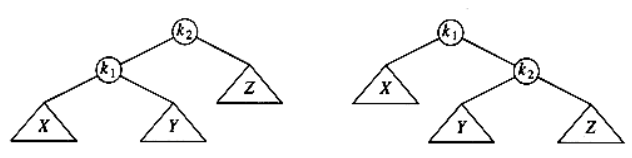
\includegraphics[width=0.8\textwidth]{rotation_example}\\
  \caption{example of rotation}%\label{}
\end{figure}
%\iffalse
%\begin{figure}
%  \centering
  % Requires \usepackage{graphicx}
%  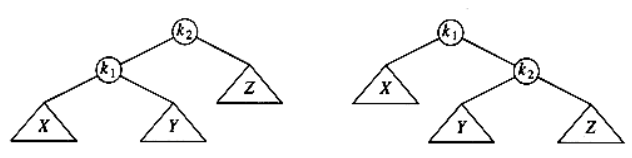
\includegraphics[width=0.8\textwidth]{rotation_example}\\
%  \caption{example of rotation}%\label{}
%\end{figure}
%\begin{figure}
%  \centering
  % Requires \usepackage{graphicx}
%  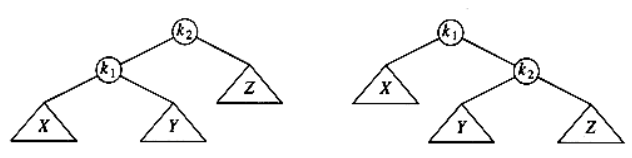
\includegraphics[width=0.8\textwidth]{rotation_example}\\
%  \caption{example of rotation}%\label{}
%\end{figure}
%Let's see how to 'rotate' it.
%\fi
% It's much easier to implement than any other balanced BSTs(e.g. Red-Black trees).
\section{Splaying}

\begin{figure}
  \centering
  % Requires \usepackage{graphicx}
  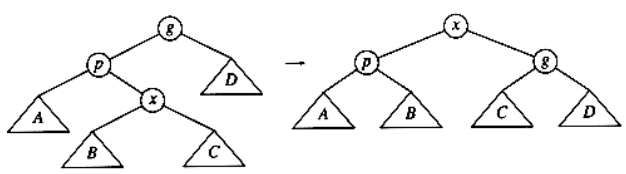
\includegraphics[width=0.8\textwidth]{zig_zag}\\
  \caption{zig-zag}%\label{}
\end{figure}

Let's come back to our splay tree. And now we want to rotate the accessed node to the root and the rotation idea used here is called 'splay'. Let $x$ be a (nonroot) node on the access path at which we are rotating. If the parent of $x$ is the root of the tree, we merely rotate $x$ and the root. Otherwise, $x$ has both a parent (p) and a grandparent (g), and there are two cases, plus symmetries, to consider. The first case is the \textbf{zig-zag} case(see Figure 2). Here $x$ is a right child and p is a left child(or vice versa). If this is the case, we first perform a left rotation on $x$ and $p$, then perform a right rotation on $x$ and $g$:
\begin{enumerate}
  \item
    Rotate $x$ and $p$, which involves only a few pointer changes:
    \begin{itemize}
       \item $x$$\rightarrow$parent = $p$$\rightarrow$parent;
       \item $p$$\rightarrow$parent = $x$;
       \item $p$$\rightarrow$right\_child = $x$$\rightarrow$left\_child;
    \end{itemize}
    \item
    Rotate $x$ and $g$, which also involves only a few pointer changes:
    \begin{itemize}
      \item $x$$\rightarrow$parent = $g$$\rightarrow$parent;
      \item $g$$\rightarrow$parent = $x$;
      \item $g$$\rightarrow$left\_child = $x$$\rightarrow$right\_child;
    \end{itemize}
\end{enumerate}
\begin{figure}
  \centering
  % Requires \usepackage{graphicx}
  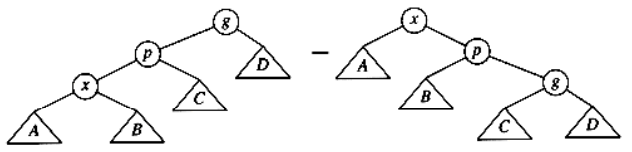
\includegraphics[width=0.8\textwidth]{zig_zig}\\
  \caption{zig-zig}%\label{}
\end{figure}
Otherwise, we have a \textbf{zig-zig} case: $x$ and $p$ are either both left children or both right children. In that case, we transform the tree on the left of Figure 3 to the tree on the right. This is done by first perform a left rotation on $p$ and $g$, then again on $x$ and $p$. We omit the pseudo code here(There will be a complete C++ implementation in the 'implementation' section).

\begin{figure}
  \centering
  % Requires \usepackage{graphicx}
  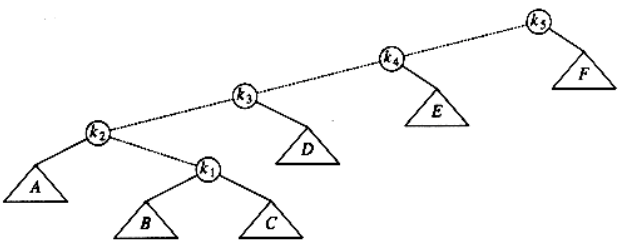
\includegraphics[width=0.8\textwidth]{step_0}\\
  \caption{init}%\label{}
\end{figure}

As an example, consider the tree on Figure 4, with a \textbf{find operation} on $k_1$:
The first step is finding $k_1$, which has no difference with the standard binary tree. Then we start the \textbf{splay} step. The first splay step is at $k_1$, and is clearly a \textbf{zig-zag}, so we perform the zig-zag rotation discussed above using $k_1, k_2$ and $k_3$. Figure 5 shows the resulting tree.

\begin{figure}
  \centering
  % Requires \usepackage{graphicx}
  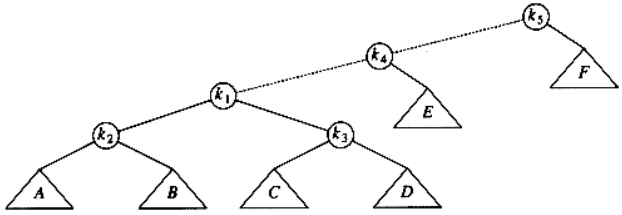
\includegraphics[width=0.8\textwidth]{step_1}\\
  \caption{step 1}%\label{}
\end{figure}

The next splay step at $k_1$ is a \textbf{zig-zig}, so we do the zig-zig rotation with $k_1, k_4$ and $k_5$, obtaining the final tree.

\begin{figure}
  \centering
  % Requires \usepackage{graphicx}
  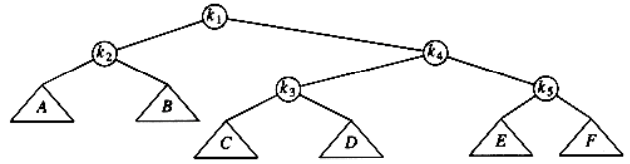
\includegraphics[width=0.8\textwidth]{step_2}\\
  \caption{final tree}%\label{}
\end{figure}

\section{Insertion and Deletion}
It's very easy to perform insertion and deletion on a splay tree. We perform insertion by first insert the node as usual, and then splay the inserted node to the root; As for deletion, we first access the node to be deleted. This put the node at the root. We now get two subtrees $T_L$ and $T_R$(left and right). If we find the largest element in $T_L$(which is easy), then this element is rotated to the root of $T_L$, and $T_L$ will now have a root with no right child. We can finish the deletion by making $T_R$ the right child.

The implementation details will be talked in the next article.

\end{document}